\documentclass[aps,prresearch,twocolumn,superscriptaddress,nofootinbib,longbibliography,floatfix]{revtex4-2}
\usepackage[T1]{fontenc}
\usepackage{amsmath,amssymb,graphicx,bm,booktabs}
\usepackage[colorlinks=true,linkcolor=blue,citecolor=blue,urlcolor=blue]{hyperref}
\newcommand{\G}{\mathcal{G}}
\newcommand{\todo}[1]{\textcolor{red}{[TODO: #1]}}

\begin{document}

\title{Photonic shake-off: leakage decay can destroy the qubit–photon bound state in passive leakage filters}

\author{Dino \v{S}krgi\'c}
\affiliation{Department of Physics, University at Buffalo, SUNY, Buffalo, New York 14260, USA}
\author{Dejan Stojkovic}
\affiliation{Department of Physics, University at Buffalo, SUNY, Buffalo, New York 14260, USA}

\date{\today}

\begin{abstract}
Placing a transmon's qubit transition in a photonic band gap and its leakage transition in a pass band turns the
waveguide into a passive leakage filter. The qubit is protected by a qubit--photon bound state, and leakage relaxes
into the band. We show that the leakage decay can also release the bound state. The doubly excited emitter, with
energy $2\Omega-\alpha$, can leave as two band photons instead of one, returning the qubit to its ground state. This
channel requires that $2\Omega-\alpha$ can be split between two pass bands. Next to a single gap edge $\omega_e$, counting
pairs from the band below the gap, this gives $\Omega<\omega_e+\alpha/2$, so only the upper half of the naive filter window is free of the channel;
pairs from non-adjacent bands add less than $10^{-4}$ on capacitively loaded lines. We derive a closed-form branching
ratio that treats the qubit's dressing exactly and the leakage decay to second order, including the interference of
the two emission orderings, and verify it against exact two-excitation dynamics to within $0.05$ in population. We
then separate what is Markovian from what is not. The criterion follows from energy conservation and does not assume
Markovian dynamics. The branching ratio requires only the leakage decay to be Markovian, and applies when the leakage
linewidth $\Gamma$ is small compared with the open two-photon window $\Delta^{(2)}$. When $\Gamma\gtrsim\Delta^{(2)}$,
bath memory suppresses the channel, by up to a factor of 25 in the range we computed. This is the regime of the only
previous study of this configuration we know of, which concluded that the cascade proceeds stepwise as in open space;
in the same model, the channel removes about a third of the bound population once $\Gamma/\Delta^{(2)}\lesssim0.5$.
For a published band-pass leakage filter, the criterion places the onset near $4.66$\,GHz, inside the reported
operating range, and the filter's own circuit model gives a loss of about $1\%$ per leakage event below it. The rule
behind the criterion, that a multiphoton channel is open when its photons can share the energy among pass-band
frequencies, also applies to pumped circuits: in a cat qubit whose buffer drains through a band-pass filter, it locates
with no fitted parameter the upper edge of a parity-degradation band, across which the measured parity recovers from
$0.12$ to $0.81$.
\end{abstract}

\maketitle

%=========================================================================================================
%\section*{Popular summary}
%Superconducting qubits sometimes leak into a
%third energy level. One elegant fix uses a structured waveguide: the qubit's frequency sits in a forbidden band, where
%it cannot radiate and is protected, while the leaked level sits in an allowed band and quickly decays back. We show that
%this decay has a hidden second route. Instead of one photon, the leaked level can emit two, and in doing so it releases
%the qubit from the protective photon cloud that the forbidden band created around it. We derive when this happens,
%how often, and why an earlier study of the same physics missed it: there, the decay was too fast for the waveguide to
%``notice'' the second route. The result is a simple design rule for structured-bath devices.

%=========================================================================================================
\section{Introduction}
%\emph{Intuitive, cross-discipline intro}
%Superconducting qubits (transmons) are supposed to use only two energy levels, 0 and 1, for the error correction algorithms. But they have a third level, 2, just above, and sometimes the qubit accidentally ends up there. This "leakage" is a nasty error for quantum error correction, so people want ways to drain level 2 back down quickly.

%A clever way to solve this is to attach the qubit to a special wire (a filter or "photonic crystal") that only lets certain frequencies of light travel through it. Tune things so the qubit's normal $1\to0$ frequency falls in a forbidden range (a "gap"), where the qubit can't emit a photon and is protected, while the $2\to1$ frequency falls in an allowed range (a "band"), where level 2 can shed a photon and drop back to 1. The wire acts like a one-way drain for the error state, and it's passive: no pulses, no control, it just works.
%However, there is a catch that has been assumed away. A qubit sitting in a gap isn't a bare, clean level. It holds onto a small cloud of light around itself, a "bound state." It's protected, but it's slightly mixed with the light in the wire. Everyone treated the leakage drain as a simple one-step process: level 2 emits one photon, lands on level 1, done, qubit intact.
%We show here that level 2 sometimes doesn't stop at level 1. It can emit two photons at once, both escaping down the wire, and the qubit drops all the way to 0. The protected state gets thrown away along with the error. The name "shake-off" is borrowed from atomic physics, where an electron gets shaken loose when an atom suddenly changes.
%The two photons together have to carry away the energy of level 2, and both have to fit into frequencies the wire allows. That works only when the qubit sits close to the edge of the gap, within half the qubit's anharmonicity. So the "safe operating window" for these filters is really only half as wide as people thought.
%An earlier study~\cite{NikolopoulosLambropoulos2000} looked at essentially this situation and concluded the decay just goes step by step, as in empty space. The new paper redoes their calculation and finds the two-photon channel was open there too, but hidden. When level 2 decays very fast compared with how "wide" the two-photon escape route is, the system has no time to use that route, so it gets suppressed, by about twelvefold at their parameters. In a slower, gentler regime the effect comes back strongly, removing over a third of the protected state.

%A leakage-filter experiment~\cite{Thorbeck2024} has part of its stated operating range, below about 4.66 GHz, in the region where this effect is allowed.
%Designers of such filters should keep the qubit in the upper half of the window.
%Quantum simulators built on these bound states should account for it.
%It produces a testable fingerprint: pairs of photons whose energies add up to the level-2 energy, which can be detected at the output.


%\emph{Leakage and structured baths.}
Transmons are weakly anharmonic ladders, and population leaking into $|2\rangle$ is a correlated, non-Pauli error that
surface codes handle poorly~\cite{Battistel2021,Miao2023,Acharya2024}. In a recent below-threshold surface-code
experiment, correlated errors, including leakage, made up an estimated $17\%$ of the error budget, and such leakage must be addressed for operating surface codes with transmon qubits~\cite{Acharya2024}. Active
leakage-reduction units remove $|2\rangle$ with drives~\cite{Battistel2021,Marques2023,Lacroix2025,Yang2024}, which builds on the setup of 
all-microwave reset~\cite{Magnard2018}. A passive alternative, on the other hand, uses the qubit's own environment, and engineered dissipation is
by now a standard resource~\cite{Harrington2022,Harrington2019}. Filtered environments already protect qubits
during readout~\cite{Sete2015}. If the qubit transition lies in a stop band or photonic band gap and the
leakage transition lies in a pass band, $|2\rangle$ relaxes quickly while $|1\rangle$ is protected. This geometry was
realized in a band-gap metamaterial~\cite{Mirhosseini2018}, built as an always-on filter with a high-order band-pass
filter and a cold resistor~\cite{Thorbeck2024}, and implemented with flux-activated coupling to a metamaterial
waveguide~\cite{Kim2025}. In a disordered transmon array, a discrete analogue moves leakage instead: frequencies are tuned so that the
doubly excited states $|20\rangle$ and $|02\rangle$ of neighbouring sites are degenerate, and the leakage hops as a
bound doublon through the virtual state $|11\rangle$ to a dissipative site, while detuned qubit states stay
localized~\cite{MartinVazquez2025,Tolppanen2026}.

%\emph{The assumption.}
All of these treat the decay of $|2\rangle$ as a one-photon process, $|2\rangle\to|1\rangle$ plus a band photon, with the
protected qubit left intact. But a qubit inside a gap is not a bare level. It forms a qubit--photon bound
state~\cite{JohnWang1990,JohnQuang1994,KofmanKurizkiSherman1994,Lambropoulos2000RPP,LiuHouck2017,Sundaresan2019,Ferreira2021,Scigliuzzo2022,Sheremet2023},
the same object that underpins band-gap quantum simulators~\cite{Zhang2023}: an eigenstate with bare weight
$Z_1<1$ and an evanescent photon cloud. Whether this dressed state survives its own emitter's cascade is not settled by
one-photon reasoning.

%\emph{What was known.}
For a three-level ladder atom at the edge of an isotropic photonic band gap, Nikolopoulos and Lambropoulos (N\&L) solved
the two-excitation dynamics exactly~\cite{NikolopoulosLambropoulos2000}, building on their treatment of structured
reservoirs with multiple excitations~\cite{BayLambropoulosMolmer1997,Lambropoulos2000RPP}. With the upper transition in the gap, they
found that a ``direct'' two-photon process makes the upper bound state metastable once the two-photon detuning
$\Delta^{(2)}$ is positive. For the configuration relevant here, with the upper transition in the band, they concluded
that ``it seems preferable for the system to decay via the stepwise process rather than the two-photon process$\ldots$
This is no different from the behavior of a ladder system in open space''~\cite{NikolopoulosLambropoulos2000}. Dalton
and Garraway stressed that both emission orderings must be kept when two transitions share one
reservoir~\cite{DaltonGarraway2003,GarrawayDalton2006}; their examples place both transitions at the same Lorentzian
feature of the reservoir, so the case of an upper transition in a band and a bound lower one does not arise. Two-excitation physics of two-level emitters on
lattices, including states with one bound and one free photon and their excitation by two-photon scattering, is well
established~\cite{Longo2010,ShiChangCirac2015,ShiWuGonzalezTudelaCirac2016,Calajo2016,SanchezBurillo2017,Calajo2019,Trivedi2021},
and a bound excitation can be released into the band by sweeping the emitter frequency~\cite{CastilloMoreno2025} or
trapped and released by a waveguide boundary~\cite{Tufarelli2013}.
Three-level emitters that radiate photon pairs have been studied in gapless waveguides, both in theory~\cite{SanchezBurillo2014,SanchezBurillo2016,Chuikin2026,Gao2024,Rieck2025},
including a resolvent treatment of the decay of a three-level transmon into a broadband one-dimensional cavity with a
Gaussian density of states~\cite{Greenberg2026}, and in experiment, where the cascade photons of a transmon are correlated~\cite{Gasparinetti2017}. A recent no-go
theorem shows that a Kerr-nonlinear mode cannot host a two-photon bound state in a continuum whose spectral density
vanishes only at isolated points~\cite{Chang2026}; true gaps are exactly the case it excludes.

%\emph{This work.}
We show that the N\&L conclusion does not hold in general. The leakage decay of a transmon can release its own bound
state, a process we call photonic shake-off. We give here an energy criterion: the channel is open when the two-photon joint density of states seen by the emitter is
nonzero at $2\Omega-\alpha$; next to one edge, counting the adjacent band, $\Omega<\omega_e+\alpha/2$. Furthermore, a closed-form branching ratio is calculated, exact in the qubit's dressing and second order in the leakage decay, with the
interference of the two emission orderings, validated against exact two-excitation dynamics to within $0.05$ in
population. Finally, we address the separation of Markovian and non-Markovian content. The criterion needs no Markov assumption. The branching
ratio needs only the leakage decay to be Markovian, $\Gamma\ll\Delta^{(2)}$, a condition on scales rather than a sharp
boundary. Outside that regime, bath memory suppresses the channel. In
N\&L's own model and at their parameters, the suppression is twelvefold, which is why the cascade looked stepwise.

The consequences are concrete. Only the upper half of the naive filter window is free of shake-off; in the lower half
the loss per leakage event ranges from about $1\%$ in a published filter to tens of percent next to a bright band edge.
For the device of Ref.~\cite{Thorbeck2024} the onset falls near $4.66$\,GHz, inside its reported operating range.
Capacitively loaded lines keep a clean window at every band index, while inductively loaded ones do not. The
kinematic rule behind the criterion, that a multiphoton channel is open exactly when its photons can share the energy
between pass bands, is not specific to leakage filters. Filters in superconducting circuits are specified by their
one-photon response at a few frequencies, while the protection they give a nonlinear or pumped element depends on where
the photons of every multiphoton process land. For pumped circuits, sampling the bath at each emitted frequency is
standard, and the map of these frequencies has been used to constrain the bandwidth of a Purcell-like filter, with the bath
taken flat~\cite{Carde2024}. In a pumped cat qubit whose buffer drains through a band-pass
filter~\cite{Putterman2025}, it places the upper end of a parity-degradation band, whose extent and dip the authors'
discrete-resonance model leaves unexplained, at the measured position with no fitted parameter (Sec.~\ref{sec:disc}).

%\emph{Terminology.}
Formally, the process is a configuration interaction of the Fano type~\cite{Fano1961}: the doubly excited emitter is a
discrete state embedded in two continua, one-photon-plus-bound-state and two-photon. It resembles laser-induced
autoionization~\cite{RzazewskiEberly1981,LambropoulosZoller1981,KnightLauderDalton1990}, except that the embedding
photon is emitted spontaneously by the same emitter. We avoid ``ionization'' of the transmon, which in circuit QED context
refers to the drive-induced escape of the phase particle from the cosine
well~\cite{Shillito2022,Cohen2023,Dumas2024}. Here the transmon stays in its well and a photon is released.

%=========================================================================================================
\section{Model}\label{sec:model}

%\subsection{Bath: a periodically loaded transmission line}
We consider a transmission line (capacitance $c_\ell$ per length, wave speed $v$) loaded every period $a$ with a shunt
capacitor $C_0$. The flux obeys $W(y)\Phi_{tt}=v^2\Phi_{yy}$ with $W=1+2r_0\sum_n\delta(y-na)$ and $2r_0=C_0/c_\ell$.
We use units $a=v=c_\ell=1$. Eliminating the slopes across one period gives a recursion for the field on the loading
points (Appendix~\ref{app:green}),
\begin{equation}
u_{n+1}+u_{n-1}=2z(\omega)\,u_n,\qquad z_{C}=\cos\omega-r_0\omega\sin\omega .
\label{eq:disp}
\end{equation}
This is the textbook capacitively loaded periodic line~\cite{Pozar,Brillouin}. Since this line includes scatterers whose response scales with frequency, we label it the 'kinetic crystal' (KC). Placing shunt
inductors $L_0$ periodically instead gives
\begin{equation}
z_{L}=\cos\omega+\frac{V_0}{2\omega}\sin\omega,\qquad V_0=\frac{\ell_\ell a}{L_0},
\label{eq:dispL}
\end{equation}
which we label KP. This is the Kronig-Penney model: each inductor adds a slope jump $+V_0u_n$ of fixed strength, the
analogue of a $\delta$-function potential, and the $1/\omega$ comes from converting slope to field across a cell. The
inductor's susceptance $1/\omega L_0$ falls with frequency, so the scatterers fade and the gaps close at high frequency.
A shunt capacitor instead adds to the kinetic ($\dot\Phi^2$) term; its jump, $-2r_0\omega^2u_n$, grows with frequency,
so the gaps widen. Bands satisfy $|z|\le1$, with $\lambda=e^{iq}$ and $\cos q=z$. Each band edge is of one of two
kinds. At a Bragg edge ($\omega=n\pi$) the Bloch wave has a node on every loading point, so the loading does
not act and the edge is fixed by the cell length alone. At a kinetic edge ($z=\pm1$ with $\sin\omega\neq0$) the
field is largest on the loading points and the loading sets the edge. Each capacitive band is bounded by a Bragg edge
below and a kinetic edge above; the capacitive bands narrow as $2/(r_0\omega)$ and the gaps approach $\pi$, while the
inductive line does the opposite.

%\textit{Green's function.} 
A source at loading point $m$ adds one slope discontinuity, which gives the exact retarded
Green's function on the loading points,
\begin{equation}
G_{nm}(\omega)=\frac{\sin\omega}{\omega}\,\frac{\lambda^{|n-m|}}{\lambda^{-1}-\lambda},\qquad |\lambda(\omega+i0)|<1 .
\label{eq:green}
\end{equation}
In a band, $G_{00}=i\sin\omega/(2\omega\sin q)$ is purely imaginary. The Purcell factor $P=\sin\omega/\sin q$ vanishes
at Bragg edges (dark) and diverges at kinetic edges (bright). The coupling capacitor $C_g$ loads the
emitter's own site. We include it exactly through a one-site Dyson equation, $\G_d=G_{00}/(1-C_g\omega^2G_{00})$, the
lattice analogue of the coupling-capacitor renormalization of continuum circuit
QED~\cite{Malekakhlagh2017,Gely2017,ParraRodriguez2018} and of the Koster--Slater impurity~\cite{KosterSlater1954,Economou2006}. Such beyond-tight-binding terms are known to
shift band edges and open gaps in circuit-QED lattices~\cite{Lee2026}, which is why we keep them.

%\subsection{Emitter}
A transmon (transition $\Omega$, anharmonicity $\alpha>0$, total capacitance $C_\Sigma$) couples through $C_g$ to one
loading point. In the rotating-wave approximation (Appendix~\ref{app:circuit}),
\begin{equation}
H=\sum_n E_n|n\rangle\langle n|+\sum_k\omega_kb_k^\dagger b_k+\sum_k g_k\big(c^\dagger b_k+b_k^\dagger c\big),
\label{eq:H}
\end{equation}
with $E_n=n\Omega-\tfrac\alpha2n(n-1)$, $c=\sum_n\sqrt n|n-1\rangle\langle n|$, $g_k=\tfrac12\sqrt{\kappa\Omega\omega_k}\,F_k$
and $\kappa=C_g^2/C_\Sigma$~\cite{Koch2007,Blais2021}. The bath enters through the emission function
\begin{equation}
\Gamma_{\rm ph}(\omega)\equiv2\pi\sum_kg_k^2\delta(\omega-\omega_k)=\kappa\Omega\omega^2\,\mathrm{Im}\,\G_d(\omega),
\label{eq:gph}
\end{equation}
the lattice form of the admittance formula for transmon emission~\cite{Houck2008}.
For a linear emitter the full non-RWA problem is solved by the pole equation $\Omega^2-E^2=\kappa E^4\G_d(E)$; we use it
to calibrate the RWA frequency so that the RWA dressed qubit coincides with the exact pole.

%\textit{One quantum.}
The qubit resolvent $G_1(z)=[z-\Omega-\Sigma(z)]^{-1}$, with $\Sigma(z)=\sum_kg_k^2/(z-\omega_k)$, has
a pole $E_{b1}$ in the gap with weight $Z_1=[1-\Sigma'(E_{b1})]^{-1}$. The band continuum carries the rest,
$1-Z_1=\int_{\rm band}A_1(\varepsilon)\,d\varepsilon$. The bound state is a pole outside the continuum, so it is
intrinsically non-Markovian; we never treat the qubit's coupling to the bath perturbatively.

%=========================================================================================================
\subsection{Two channels and the energy criterion}\label{sec:criterion}

\begin{figure*}[t]
\centering
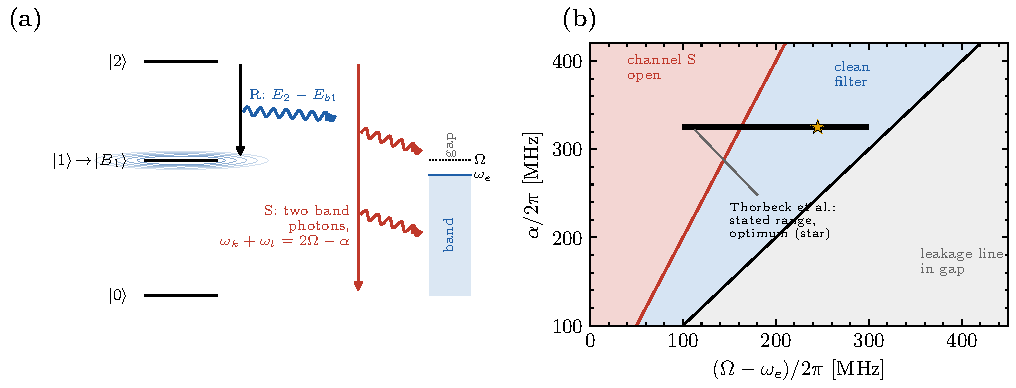
\includegraphics[width=\textwidth]{fig_schematic.pdf}
\caption{\label{fig:schematic}Left: A leakage event $|2\rangle$ of a transmon whose qubit transition is bound in a gap
above the band edge $\omega_e$. In the retained channel R, one band photon at $E_2-E_{b1}$ leaves and the qubit stays in
its bound state $|B_1\rangle$. In the shake-off channel S, two band photons with $\omega_k+\omega_l=2\Omega-\alpha$
leave and the emitter returns to $|0\rangle$, releasing the photon cloud. Right: Design map from Eq.~\eqref{eq:threshold}:
channel S is open for $\Omega-\omega_e<\alpha/2$ (red), the filter is clean for $\alpha/2<\Omega-\omega_e<\alpha$
(blue), and above $\alpha$ the leakage line is itself in the gap. The bar and star mark the stated operating range and
optimum of the passive filter of Ref.~\cite{Thorbeck2024} (edge $4.5$\,GHz, $\alpha/2\pi=325$\,MHz).}
\end{figure*}

Start from a leakage event, $|2;\mathrm{vac}\rangle$, with energy $E_2=2\Omega-\alpha$. Its decay has two kinds of final
states (Fig.~\ref{fig:schematic}). In the retained channel R, the final state is $|B_1;k\rangle$: the qubit stays in
its bound state and one leakage photon leaves. In the shake-off channel S, the final state is $|0;k,l\rangle$: two
band photons leave and the emitter returns to its ground state.

Energy conservation in channel S requires $\omega_k+\omega_l=E_2$, with both photons emitted at the emitter's loading
point. What counts is therefore the local density of states there, weighted by the coupling, which is the emission
function $\Gamma_{\rm ph}$ of Eq.~\eqref{eq:gph}. Define the two-photon joint density
\begin{equation}
\rho_2(E)=\int d\omega\,\Gamma_{\rm ph}(\omega)\,\Gamma_{\rm ph}(E-\omega).
\end{equation}
It differs from the bulk two-photon density of states only at isolated zeros of $\Gamma_{\rm ph}$ (Bragg points, or
nodes of a giant-atom form factor), which do not change where $\rho_2$ vanishes. Our criterion is that channel S is open
when $\rho_2(E_2)>0$, i.e.\ when $E_2$ lies in the sum set $\mathcal B+\mathcal B$ of the pass bands. The two-photon
amplitude, Eq.~\eqref{eq:M}, vanishes only at isolated frequencies and does not close the channel, but it can make
it very weak (below). For a transmon the leakage line sits below the qubit, so the relevant edge is the lower edge $\omega_e$ of the
qubit's gap, which is the top of the band below. If only that band can absorb both photons,
\begin{equation}
\text{channel S open}\iff\Omega<\omega_e+\alpha/2 .
\label{eq:threshold}
\end{equation}
The naive filter window $(\omega_e,\omega_e+\alpha)$ therefore splits into a lower half where shake-off is allowed and a
clean upper half. The width $\alpha/2$ cannot be exceeded by any band structure. Over a contiguous range of qubit
frequencies in which the leakage line stays in one pass band, if that range is wider than $\alpha/2$, then for some
$\Omega$ the midpoint $\Omega-\alpha/2$ also lies in the band, and two photons at the midpoint conserve energy. Filter
design can therefore suppress the rate in the lower half, but cannot remove the channel there. Higher levels obey a staircase: $|n\rangle$ can release the bound state if
$\Omega<\omega_e+(n-1)\alpha/2$. The criterion uses only energy conservation and the band structure, so it does not
rely on a Markov approximation. Non-Markovian effects change how much population takes the open channel, not whether or not it is open.

%\emph{Non-adjacent pairs.} 
Eq.~\eqref{eq:threshold} counts only pairs from the band directly below the gap. In the
upper half, pairs from other bands can still conserve energy, for instance one photon in band 0 and one in band 2 next
to gap 2 of the capacitive line, so $\rho_2(E_2)$ need not vanish there. These pairs are strongly suppressed. Both
photons are far from the qubit, at detunings $-\Delta$ and $\Delta-\alpha$ with $\Delta\gg\alpha$, and the two
emission orderings nearly cancel: $G_1(\omega)+G_1(E_2-\omega)\simeq\alpha/\Delta^2$, so the rate carries a factor
$(\alpha/\Delta^2)^2$. Evaluating Eq.~\eqref{eq:G2} band pair by band pair, the non-adjacent loss in the upper half of
the capacitive line is below $2\times10^{-6}$ for gaps 1-2, $10^{-5}$ for gap 3 and $10^{-4}$ for gap 4. The
inductive bands are wide, so the photons need not be far from the qubit, and non-adjacent pairs dominate the loss
above the adjacent threshold (Sec.~\ref{sec:results}). We call the upper half clean when, as on the capacitive
line, the non-adjacent residual is negligible.

%=========================================================================================================
%\section{Branching ratio}\label{sec:theory}

In the channel R, only the bare-$|1\rangle$ component of $B_1$ couples, so the vertex is $\sqrt{2Z_1}\,g_k$ and
\begin{equation}
\Gamma_R=2Z_1\,\Gamma_{\rm ph}(E_2-E_{b1}).
\end{equation}

For channel S, we work to second order in the leakage vertex and to all orders in the qubit's coupling to the bath.
Either photon can be the leakage photon, so the amplitude has both orderings~\cite{GoeppertMayer1931,BreitTeller1940,DaltonGarraway2003},
\begin{equation}
M_{kl}=\sqrt2\,g_kg_l\,\big[G_1(\omega_l)+G_1(\omega_k)\big],\qquad\omega_k+\omega_l=E_2 .
\label{eq:M}
\end{equation}
Summing $2\pi|M_{kl}|^2\delta(E_2-\omega_k-\omega_l)$ over distinct pairs gives
\begin{multline}
\Gamma_{S}=\frac1\pi\!\int\!d\omega\,\Gamma_{\rm ph}(\omega)\Gamma_{\rm ph}(E_2-\omega)\\
\times\Big\{|G_1(\omega)|^2+\mathrm{Re}\,G_1(\omega)G_1^*(E_2-\omega)\Big\}.
\label{eq:G2}
\end{multline}
The first term is the direct process and the second the exchange (interference) term. The exchange term is comparable
to the direct one, and its sign depends on the bath.

After the decay, the bare qubit population and the loss per leakage event are
\begin{equation}
P_1=Z_1\,\frac{\Gamma_R}{\Gamma_R+\Gamma_{S}},\qquad L\equiv1-\frac{P_1}{Z_1}=\frac{\Gamma_{S}}{\Gamma_R+\Gamma_{S}} .
\label{eq:P1}
\end{equation}

Using $|G_1|^2\Gamma_{\rm ph}=2\pi A_1$, the direct term equals
$2\int A_1^{\rm band}(\varepsilon)\,\Gamma_{\rm ph}(E_2-\varepsilon)\,d\varepsilon$: the leakage decay can end in any
eigenstate of the dressed qubit, weighted by its bare-$|1\rangle$ content and by the photon density at the complementary
frequency. Consider the limiting cases. 
For flat $\Gamma_{\rm ph}$ and with no exchange, $P_1=Z_1^2$, i.e.\ $L=1-Z_1$. The bare $|1\rangle$ left behind is projected
onto the dressed states, as in sudden shake-off in atoms~\cite{Aberg1967,SchneiderChocianRost2002}. Furthermore, for $\rho_2(E_2)=0$: $L=0$, the adiabatic limit.
Finally, at a bright edge the final density diverges and the exchange term can add, so $L>1-Z_1$.

The shake-off ratio $L/(1-Z_1)$ is therefore the natural measure. Since $\Gamma_R\propto\kappa$ and
$\Gamma_S\propto\kappa^2$, $L=O(\kappa)$, the same order as the qubit's own dressing $1-Z_1$, implying that weaker coupling at fixed
detuning does not remove the effect.

%=========================================================================================================

The bath is strongly structured, so a natural question to ask is to what extent Eq.~\eqref{eq:P1} describes Markovian dynamics.
Structure of the bath is not the same as memory~\cite{Lambropoulos2000RPP,GonzalezTudelaCirac2017,Malekakhlagh2016}. A decay is
Markovian when the density of final states is smooth on the scale of the
decay rate, at the energies where the decay happens. We make two different choices for two different processes.
First, the qubit's dressing is treated exactly. The bound state is a pole outside the continuum, which is the most non-Markovian
object the bath produces, and it enters only through the exact resolvent $G_1$ and its residue $Z_1$.
Second, the leakage decay is treated in a Wigner-Weisskopf (golden-rule) approximation~\cite{CohenTannoudji1992}. This requires the leakage line
$E_2-E_{b1}$ to sit inside a band, away from its edges by more than the leakage linewidth $\Gamma=\Gamma_R+\Gamma_S$,
and the two-photon energy to sit above threshold by more than $\Gamma$. The second condition is
\begin{equation}
\Gamma\ll\Delta^{(2)},
\label{eq:markov}
\end{equation}
where $\Delta^{(2)}$ is the width of the open two-photon window, the distance of $E_2$ from the edge of
$\mathcal B+\mathcal B$. This is a condition on scales, not a sharp boundary; the crossover is gradual
(Fig.~\ref{fig:markov}(b)). This is the $\Delta^{(2)}$ of Ref.~\cite{NikolopoulosLambropoulos2000}; next to one edge,
$\Delta^{(2)}=2(\omega_e+\alpha/2-\Omega)$ up to dressing shifts.

\begin{figure*}[t]
\centering
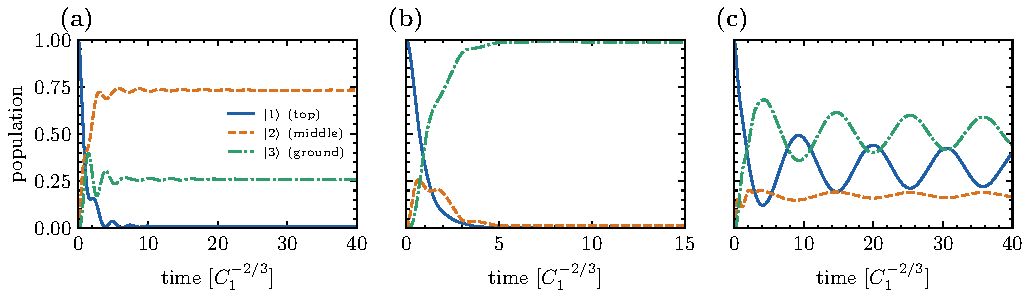
\includegraphics[width=\textwidth]{fig_nl2000_repro.pdf}
\caption{\label{fig:nlrepro}Reproduction of Figs.~4(a), 4(b) and 5(a) of Ref.~\cite{NikolopoulosLambropoulos2000}:
populations of the top ($|1\rangle$, solid), middle ($|2\rangle$, dashed) and ground ($|3\rangle$, dash-dotted) levels
of the ladder atom versus time, in N\&L's labelling, where their middle level is our qubit level. Both transitions
couple to the same isotropic band-edge reservoir with $C_2=1.5\,C_1$; detunings $\delta_{12}$, $\delta_{23}$ are measured
from the band edge, positive into the band. We use their discretization ($N=150$ modes, cutoff $\omega_u=10$, quadratic
mode spacing) and units ($C_1^{2/3}$ for energy, $C_1^{-2/3}$ for time). (a)~$\delta_{12}=C_2^{2/3}$,
$\delta_{23}=-C_1^{2/3}$: upper transition in the band, lower one bound, the configuration of this paper. Channel S is
open ($\Delta^{(2)}=0.31$), yet the middle level keeps $0.73$ of the population against a bound weight $Z=0.80$; the
cascade looks stepwise because memory suppresses the channel (Fig.~\ref{fig:markov}). (b)~$\delta_{12}=2C_2^{2/3}$,
$\delta_{23}=3C_1^{2/3}$: both transitions in the band, ordinary cascade to the ground state. (c)~$\delta_{12}=-2C_2^{2/3}$,
$\delta_{23}=2C_2^{2/3}$: the mirror configuration, upper transition in the gap, with $\Delta^{(2)}=0$; the surviving
population oscillates between the top and ground levels through the direct two-photon process.}
\end{figure*}

\begin{figure*}[t]
\centering
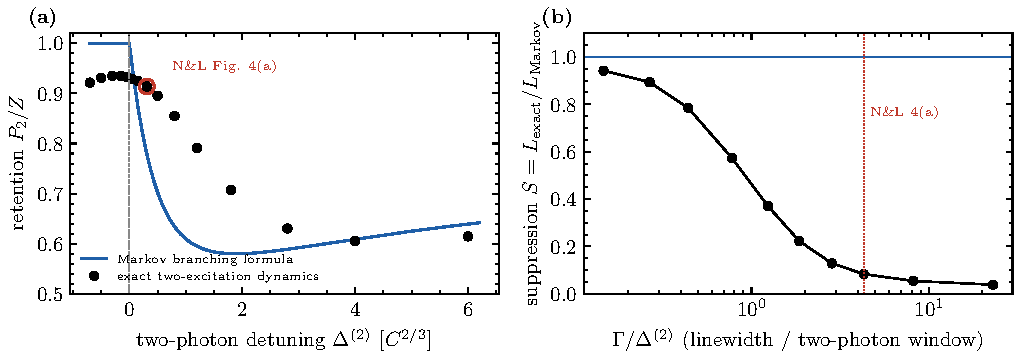
\includegraphics[width=0.9\textwidth]{fig_markov.pdf}
\caption{\label{fig:markov}Markovian limit of photonic shake-off in the model of Ref.~\cite{NikolopoulosLambropoulos2000}
($C_2=1.5\,C_1$), with the lower transition bound at $\delta_{23}=-1$ (bound weight $Z=0.80$) and the upper transition
scanned into the band. (a)~Retention $P_2/Z$ of the lower bound state after the cascade versus the two-photon detuning
$\Delta^{(2)}=\delta_{12}+\delta_{23}$; channel S is open for $\Delta^{(2)}>0$ (dashed line). Markers: exact
two-excitation dynamics, averaged over $t\in[40,60]$ ($N=250$, $\omega_u=20$; $N=400$--$450$, $\omega_u=30$ for
$\Delta^{(2)}\ge2.8$). Line: Markov branching formula, Eqs.~\eqref{eq:G2} and \eqref{eq:P1}, with the model's
self-energy $\Sigma(y)=-C/\sqrt{-y}$. The circled point is their Fig.~4(a). Below threshold the exact retention is
$b_0=0.93$ rather than 1, because the upper level decays on the time scale on which the lower bound state forms; this
deficit is unrelated to channel S. Just above threshold the exact retention stays near $b_0$ while the formula drops;
deep in the band the two agree. (b)~Suppression factor $S=L_{\rm exact}/L_{\rm Markov}$, with
$L_{\rm exact}=1-(P_2/Z)/b_0$ and $L_{\rm Markov}=1-P_2^{\rm Markov}/Z$, versus the ratio of the Markov leakage linewidth
$\Gamma=\Gamma_R+\Gamma_S$ to the open two-photon window $\Delta^{(2)}$. $S$ rises monotonically from $0.04$ to $0.94$ as
$\Gamma/\Delta^{(2)}$ falls from $23$ to $0.15$; at N\&L's Fig.~4(a) (dashed line, $\Gamma/\Delta^{(2)}=4.3$) the loss is
suppressed twelvefold.}
\end{figure*}

The isotropic model of Ref.~\cite{NikolopoulosLambropoulos2000} has a band-edge density of states $\propto1/\sqrt x$, so
it reaches deep into the non-Markovian regime. N\&L number the levels from the top: their $|1\rangle$, $|2\rangle$ and
$|3\rangle$ are our $|2\rangle$, $|1\rangle$ and $|0\rangle$. Their $P_2$ is therefore the population of our qubit
level, and $P_2/Z$, with $Z$ its bound weight, is the retention, the analogue of $P_1/Z_1$. We reproduce their dynamics curve for curve with their discretization
(Fig.~\ref{fig:nlrepro} and Appendix~\ref{app:nl}). Their Fig.~4(a) is our configuration: upper transition in the band,
lower in the gap, with $\Delta^{(2)}>0$, so channel S is open. In the exact dynamics the middle level nonetheless keeps
$0.73$ of the population against a bound weight $Z=0.80$, so the cascade looks almost stepwise. We then keep the
lower transition bound ($\delta_{23}=-1$) and scan the upper transition into the band (Fig.~\ref{fig:markov}).

Below threshold ($\Delta^{(2)}<0$) channel S is closed. The retention is $0.93$, not $1$, because the upper level
decays on a time scale comparable to the formation of the lower bound state. This deficit has nothing to do with
channel S.
Just above threshold the exact loss is far below the Markov prediction. At N\&L's Fig.~4(a), $\Delta^{(2)}=0.31$,
the exact retention is $0.914$ against $0.779$ from Eq.~\eqref{eq:P1}, and the loss attributable to channel S is only
$2\%$. There $\Gamma/\Delta^{(2)}=4.3$, and the upper transition is itself non-Markovian ($\Gamma$ comparable to its
detuning from the edge).
Deeper in the band the Markov formula takes over. For $\Gamma/\Delta^{(2)}=0.27$ the exact and Markov retentions
are $0.606$ and $0.609$. Normalized to $b_0$, the exact loss is $0.32$--$0.35$ for $\Gamma/\Delta^{(2)}=0.15$--$0.44$,
against $0.36$--$0.41$ from Eq.~\eqref{eq:P1}; without the normalization, the raw retentions agree with
Eq.~\eqref{eq:P1} to within $0.04$ over the same range.

The suppression factor in Fig.~\ref{fig:markov}(b) rises monotonically from $0.04$ to $0.94$ as $\Gamma/\Delta^{(2)}$
falls from $23$ to $0.15$. We interpret this as a memory effect. The open two-photon window has width $\Delta^{(2)}$, so
the two-photon continuum, measured from its threshold, has a correlation time of order $1/\Delta^{(2)}$. A level that
decays faster than this cannot resolve the window and leaks predominantly through the stepwise channel. Non-Markovianity
does not create photonic shake-off; it hides it. N\&L's conclusion that the cascade is stepwise ``as in open space''
reflects the parameter point they examined, not the configuration.

For the devices of Sec.~\ref{sec:results}, $\Gamma_{\rm free}/\Omega\approx1\%$ and
Eq.~\eqref{eq:markov} holds except near threshold. Correspondingly, Eq.~\eqref{eq:P1} matches the exact dynamics to
within $0.05$ everywhere, and the largest deviations sit at $f=(\Omega-\omega_e)/\alpha\approx\tfrac12$. There the step
predicted by Eq.~\eqref{eq:P1} is smeared over a width set by $\Gamma$, which leaves a residual loss of a few percent in
the clean half.

In summary, the properties of photonic shake-off differ in how much they rely on Markovianity. The criterion
$\rho_2(E_2)>0$ rests on energy conservation, and holds in the exact dynamics of both models up to the leakage
linewidth: because $|2;\mathrm{vac}\rangle$ has an energy spread $\Gamma$, the threshold is smeared over a width
$\Gamma$. The bound state enters only through the exact resolvent, so the qubit's dressing is never approximated. The
branching ratio, Eq.~\eqref{eq:P1}, together with its exchange term and the scaling $L=O(\kappa)$, is a statement about
the Markovian limit, Eq.~\eqref{eq:markov}. Near threshold it is not a bound in either direction: on the open side
memory suppresses the loss, and on the closed side the smearing leaves a residual of a few percent.


%=========================================================================================================
\begin{figure*}[!t]
\centering
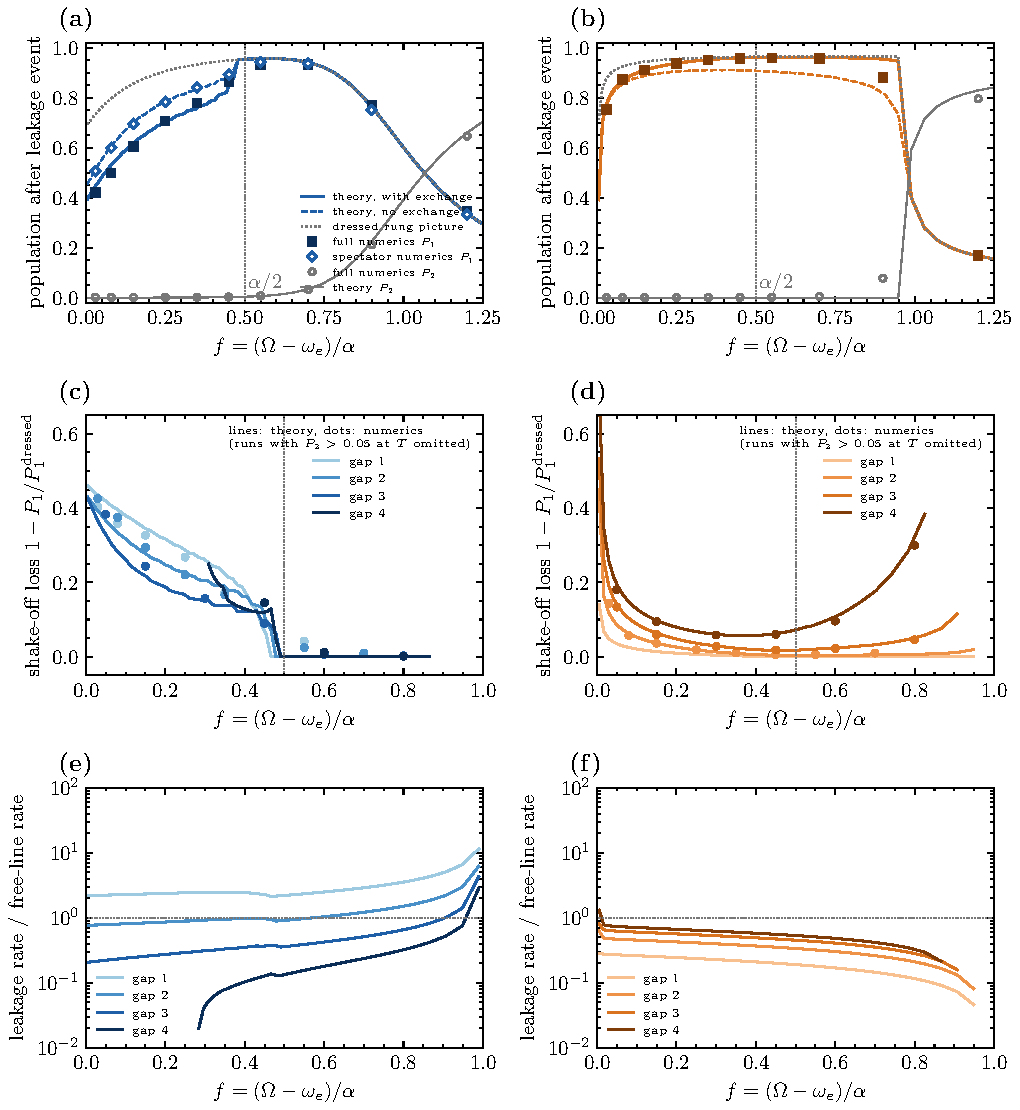
\includegraphics[width=\textwidth]{kc_selfion.pdf}
\caption{\label{fig:validation}Qubit retention and shake-off loss after a leakage event, capacitive (KC, left
column) and inductive (KP, right column) loading. The horizontal axis is the qubit's position in the naive filter
window, $f=(\Omega-\omega_e)/\alpha$, with $\omega_e$ the top of the band below the qubit's gap; channel S is
energetically open for $f<\tfrac12$ (dotted vertical line) and the leakage line itself enters the gap at $f=1$.
The device is the fixed circuit of Sec.~\ref{sec:results} ($\Gamma_{\rm free}/\Omega\approx1\%$, $C_g/C_\Sigma=0.4$,
$\alpha=0.05\,\Omega_c$). Exact populations are from the RWA two-excitation dynamics on rings of $N=140$--$250$
cells, started in $|2;\mathrm{vac}\rangle$ and averaged over $t\in[140,220]$.
(a,b)~Gap 2. Squares: exact population $P_1$ of the bare qubit level. Open circles: undecayed leakage $P_2$.
Diamonds (KC only): spectator dynamics, which omits the exchange process. Solid and dashed lines: Eq.~\eqref{eq:P1}
with and without the exchange term. Dotted grey line: dressed-rung picture, $P_1^{\rm dressed}$, in which the bound
state survives the leakage decay ($=Z_1$ when the leakage line lies in a band). Thin grey line: predicted $P_2$,
the part of $|2\rangle$ that stays bound when the leakage line approaches its band edge ($f\to1$).
(c,d)~Shake-off loss $L=1-P_1/P_1^{\rm dressed}$ for gaps 1--4 (light to dark). Lines: Eq.~\eqref{eq:P1}. Dots:
exact dynamics. Only runs in which the leakage has cleared ($P_2<0.05$ at $t=220$, in both theory and numerics) are
shown; this removes the upper end of each window, KC gap 4 for $f\lesssim0.3$, and all KP gap 1 runs, whose leakage
removal at the dark Bragg edge is too slow for the time window. In KC the loss vanishes above $f=\tfrac12$ up to
linewidth smearing; in KP, pairs from non-adjacent bands keep it finite and growing with band index.
(e,f)~Leakage-removal rate $\Gamma=\Gamma_R+\Gamma_S$ from Eq.~\eqref{eq:P1}, relative to the rate on a bare line,
$\Gamma_{\rm free}=\kappa\Omega(\Omega-\alpha)$, for gaps 1--4. KC sits at a bright kinetic edge and removes
leakage at or above the bare-line rate; KP sits at a dark Bragg edge and removes it more slowly, by up to two orders
of magnitude.}
\end{figure*}

\begin{figure*}[!htb]
\centering
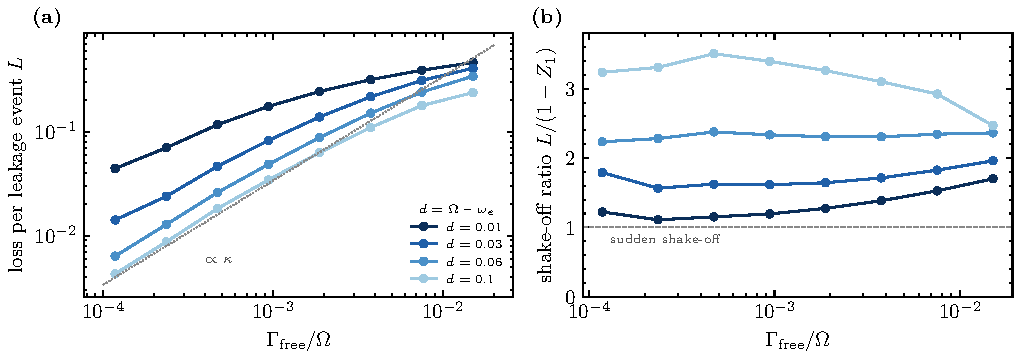
\includegraphics[width=\textwidth]{kc_selfion_scaling.pdf}
\caption{\label{fig:scaling}Scaling of the shake-off loss with the coupling strength, capacitive line, gap 2. The
coupling $\kappa$ is scaled by factors $1/64$ to $2$ at fixed $C_\Sigma$ (so $C_g\propto\sqrt\kappa$), which sweeps the
free-line linewidth at the gap edge, $\Gamma_{\rm free}/\Omega=\kappa\,\omega_e/2$, over two decades; the device of
Fig.~\ref{fig:validation} sits at $\Gamma_{\rm free}/\Omega=7.5\times10^{-3}$. The qubit is held at fixed detuning
$d=\Omega-\omega_e=0.01$, $0.03$, $0.06$ and $0.10$ above the bright kinetic edge (dark to light; about $12$, $35$, $70$
and $116$\,MHz in the units of Appendix~\ref{app:ghz}), all inside the open half of the window, $d<\alpha/2=0.129$.
Curves are Eq.~\eqref{eq:P1} with the exchange term. (a)~Loss per leakage event $L$; the dotted line is a guide
$\propto\kappa$. Away from the edge $L$ scales linearly with $\kappa$, so weaker coupling at fixed detuning does not
remove the effect. (b)~Shake-off ratio $L/(1-Z_1)$, the loss relative to the qubit's own dressing. It stays between
$1.1$ and $3.5$ over the whole range, above the sudden-shake-off value $1$ (dashed line), because the photon density at
the bright edge enhances channel S beyond the flat-band limit.}
\end{figure*}

\section{Results}\label{sec:results}

%\subsection{Validation against exact dynamics}
We solve Eq.~\eqref{eq:H} exactly in the two-excitation sector $\{|2;0\rangle,|1;k\rangle,|0;k,l\rangle\}$ on a ring
built from exact even Bloch modes, with the $C_g$ defect included and no spatial grid (Appendix~\ref{app:ring}).
Populations are averaged over $t\in[140,220]$. The mode cutoff includes every band that can absorb a photon pair at
$E_2$, so non-adjacent pairs are in the numerics. A photon returns to the emitter after circling the ring, at
$t=N/v_g$; for the bands that carry the leakage and shake-off photons this is $t\ge350$ (capacitive) and $t\ge250$
(inductive, gaps 1--3), after the averaging window. For inductive gap 4 the fastest photons return at $t\approx217$, at
the very end of the window. We show only runs in which the leakage has cleared, $P_2<0.05$ at the end of the window in
both theory and numerics. This removes the upper end of the window, where the leakage line approaches the band edge and
is partly bound; capacitive gap 4 for $f\lesssim0.3$, where the band below the gap is narrower than $\alpha$ and the
leakage line falls into the gap below; and all of inductive gap 1, where the dark Bragg edge makes leakage removal so
slow that $P_2=0.1$--$0.5$ at $t=220$. The device is a
fixed circuit placed in gap $n$ by choosing $a$, with $\Gamma_{\rm free}/\Omega\approx1\%$, $C_g/C_\Sigma=0.4$ and
$\alpha=0.05\,\Omega_c$, where $\Omega_c$ is the gap centre (Appendix~\ref{app:ghz}). In physical units, with gap centres
at $6$\,GHz on a $50\,\Omega$ coplanar host, this is $\alpha/2\pi=300$\,MHz, $C_g=25.5$\,fF, $C_\Sigma=64$\,fF and
$\Gamma_{\rm free}/2\pi=30$--$55$\,MHz at the gap edges. Gap~2 of the capacitive line spans $4.71$--$7.29$\,GHz, and its
clean window is $4.86$--$5.01$\,GHz (Table~\ref{tab:ghz}).

Figure~\ref{fig:validation} compares theory and exact dynamics.
We see that Eq.~\eqref{eq:P1} reproduces the exact dynamics to $\max|\Delta P_1|=0.03$--$0.05$ (capacitive, gaps 1-4)
and $0.005$--$0.023$ (inductive, gaps 2-4). Away from the threshold ($f\le0.3$) the loss $L$ agrees to within $15\%$
(capacitive) and $20\%$ (inductive) of its value, and the largest absolute deviations sit at $f\approx\tfrac12$, where $\Gamma\gtrsim\Delta^{(2)}$ and the step is smeared over a width $\Gamma$. 
Without the exchange term the error grows to $0.15$. The one-photon ``dressed rung'' picture assumes the bound
state survives: the leakage level decays into $|B_1\rangle$ plus one photon, so $P_1^{\rm dressed}=Z_1$ whenever the
leakage line lies in a band, which holds for all points shown (Appendix~\ref{app:amp} gives the bound-rung case). It
misses by up to $0.31$.
Finally, the spectator model, the exact dynamics without the exchange process, agrees with the direct-only formula to
$0.006$. This isolates the interference term.
Close to the edge the effect is large. In gap~1 at $f=0.03$, the qubit retains $P_1=0.43$ against $Z_1=0.72$ in
the dressed-rung picture, a shake-off loss $L=1-P_1/Z_1=0.40$ (theory $0.43$). The ground-state population, $0.57$,
also contains the photon cloud of the retained bound state, $(1-Z_1)(1-L)\approx0.17$.



%\subsection{Scaling with coupling}
At fixed detuning away from the edge, $L\propto\kappa$, with $L/(1-Z_1)\approx1.1$--$3.5$ across two decades of
$\Gamma_{\rm free}/\Omega$ (Fig.~\ref{fig:scaling}). The loss exceeds sudden shake-off everywhere in the lower half
window. At $\Gamma_{\rm free}/\Omega\sim10^{-3}$ it is $3$--$17\%$ per leakage event, depending on the detuning. The
threshold itself does not move with $\kappa$: it is fixed by energy conservation.


%\subsection{Capacitive versus inductive loading}
The criterion $\rho_2(E_2)>0$ explains the difference between the two loadings.
For capacitive loading, gaps widen with band index, so $\rho_2$ is sparse at high frequency. The filter window sits at a
bright kinetic edge, the loss is strong for $\Omega<\omega_e+\alpha/2$, and it vanishes above. The residual loss at the
best point is $4.2\%$, $1.0\%$, $0.2\%$ and $0.1\%$ for gaps 1-4, set by the leakage linewidth smearing the threshold;
non-adjacent pairs contribute less than $10^{-4}$.
For inductive loading, bands widen with index, so $\rho_2$ fills in. The window sits at a dark Bragg edge, where the
loss at the edge is weak but leakage is removed slowly. Other band pairs keep channel S open across the gap. In
Eq.~\eqref{eq:G2} they alone give $0.3$-$1\%$ (gap 2), $2$-$10\%$ (gap 3) and $9$-$23\%$ (gap 4) across the upper
half, and the minimum loss in the numerics ($0.6\%$, $1.8\%$, $5.8\%$ for gaps 2-4) grows with band index. Gap 1 has
no non-adjacent pairs, but its leakage removal is too slow to show in our time window.

The robust statement concerns $\rho_2$, not inductance as such. A left-handed line, the circuit-QED realization of an
inductively loaded bath, has a dense, gap-free spectrum above its infrared cutoff~\cite{EggerWilhelm2013,Indrajeet2020,McBroomCarroll2024,Goswami2026}
and is the extreme case with no clean window; superlattices can reopen gaps~\cite{Messinger2019}. The same band-sum
kinematics governs multiphoton down-conversion in Josephson-chain waveguides~\cite{Mehta2023}.

%=========================================================================================================

%=========================================================================================================
\section{Discussion}\label{sec:disc}
%\subsection{Experimental consequences}\label{sec:exp}

%\emph{Passive leakage filters.}
The most direct consequence is the passive leakage filter design rule. Specifically, the filter of Ref.~\cite{Thorbeck2024} is a seventh-order Chebyshev band-pass filter
with an upper cutoff of $4.5$\,GHz, coupled to a transmon with $\alpha/2\pi=325$\,MHz. Treating the cutoff as a sharp
edge, Eq.~\eqref{eq:threshold} opens channel S for $\omega_{ge}/2\pi<4.66$\,GHz. The reported optimum ($4.745$\,GHz)
lies in the clean half; the lower $60$\,MHz of the stated operating range ($4.6$-$4.8$\,GHz) does not. The edge seen by
the qubit is not sharp: the density of states on the filter's first site is a sum of seven modes broadened by the
output port. We therefore solved the two-excitation dynamics of the filter's own circuit model
(Appendix~\ref{app:thorbeck}) and computed the probability $1-L$ that an $|f\rangle$ event returns the transmon to its
dressed $|e\rangle$. With the published design values the model's $T_{1,f}$ minimum sits at $4.90$\,GHz instead of the
measured $4.745$\,GHz; we therefore shift all filter modes down by $100$--$150$\,MHz, which reproduces the measured
$T_{1,f}$ minimum and, approximately, the measured $T_{1,e}$ (Appendix~\ref{app:thorbeck}). The calibrated model gives a
peak loss $L=0.4$--$2\%$ between $4.60$ and $4.65$\,GHz, depending on $g/2\pi=15$--$25$\,MHz and on the shift. $L$ falls
below $10^{-3}$ at a frequency between $4.62$ and $4.69$\,GHz, and is $L\le10^{-4}$ at the optimum. The onset agrees
with the sharp-edge estimate; its width, a few tens of MHz, is set by the mode linewidths. Without the shift the onset
moves up with the top filter mode, and $L\approx1\%$ at $4.70$--$4.75$\,GHz, so the predicted onset is only as accurate
as the filter calibration.
Reference~\cite{Thorbeck2024} reports leakage and seepage rates but not the $|e\rangle$ retention after an $|f\rangle$
event, so its data do not constrain $L$. The prediction is a drop in $|e\rangle$ retention below about $4.66$\,GHz,
accompanied by photon pairs at the filter output.

%\emph{Bound-state simulators.} 
The same criterion applies with $\omega_e$ the top of the band below the qubit. For the
Josephson-resonator array of Ref.~\cite{Scigliuzzo2022} (band $5.219$-$6.215$\,GHz), qubit Q1 sits at most $107$\,MHz
above the band with $\alpha/2\pi\approx266$\,MHz, so channel S is open throughout its range.

%\emph{Pumped filtered baths.}
The same kinematics constrains parametrically pumped devices that dissipate through a band-pass filter. The rate of a
pump-induced transition in a structured bath follows from Floquet--Born--Markov theory, which samples the bath spectral
density at each emitted frequency~\cite{Carde2024,BenhayouneKhadraoui2025}. Reference~\cite{Carde2024} maps these
emitted frequencies for an ATS-based cat and notes that the map constrains the bandwidth of a Purcell-like filter; there the
bath is taken flat. What a filter with sharp edges adds is that a
channel switches on and off as its emitted photons enter and leave the pass band, rather than at isolated resonances.
In the dissipative cat qubit of Ref.~\cite{Putterman2025}, the buffer mode ($\bar\omega_b/2\pi\approx2.94$\,GHz when
pumped) drains through a four-pole filter with pass band $2.59$--$3.55$\,GHz, and the storage
($\bar\omega_s/2\pi\approx5.35$\,GHz) is protected outside it. A two-pump process, $2\omega_p\to\bar\omega_s+3\bar\omega_b$,
heats the storage; the authors' Floquet model places it as a discrete resonance at $\omega_p/2\pi=7.12$--$7.16$\,GHz, but the
measured storage parity is degraded over the whole range $7.10$--$7.39$\,GHz, with a deep dip near $7.35$\,GHz that the
authors leave unexplained and tentatively attribute to the filter's internal modes~\cite{Putterman2025}. If one of the
three photons is emitted into the filter continuum rather than into the buffer resonance, energy conservation puts it at
$\omega_3=2\omega_p-\bar\omega_s-2\bar\omega_b$, and the channel is open exactly while $\omega_3$ lies in the pass band.
With the measured buffer frequency at each pump frequency and no fitted parameter, $\omega_3$ leaves the upper band edge
at $\omega_p/2\pi=7.41$--$7.42$\,GHz; the measured parity recovers from $0.12$ at $7.387$\,GHz to $0.81$ at $7.428$\,GHz
(Appendix~\ref{app:cat}). Away from the discrete resonance, the deepest degradation, the dip near $7.35$\,GHz, lies
where $\omega_3$ approaches the filter's upper-edge mode at $3.464$\,GHz; its exact position relative to that mode is not
resolved by the data. Because $\omega_3$ tunes at twice the pump slope, the rule predicts a degraded band half the filter
bandwidth wide in pump frequency (more generally, $W/n$ for a process that absorbs $n$ pump photons and emits one filter
photon, with $W$ the filter bandwidth), $6.90$--$7.42$\,GHz, where a discrete-resonance search predicts a line a few MHz wide;
the published scan covers its upper $300$\,MHz. It also predicts an emission line at $\omega_3$ at the filter output, a
second recovery below $\omega_p/2\pi\approx6.90$\,GHz, and a shift of the whole band with $\bar\omega_b$. For frequency allocation in filtered, pumped circuits, the condition is that the leftover photon of every
low-order pumped process lies outside the pass band, not merely away from the buffer resonance.

%\emph{Heralding.} 
Shake-off emits photon pairs whose energies sum to $E_2$, while channel R emits single photons at
$E_2-E_{b1}$. Pair coincidences at the output, measurable with the techniques used for transmon cascade
photons~\cite{Gasparinetti2017}, herald the release of the bound state.

%\emph{Error correction.} 
For an error-correcting code, ending in $|0\rangle$ instead of $|1\rangle$ after a leakage event
is not a new error: the leaked qubit has already lost its information, and either outcome returns it to the
computational subspace. The effect matters where the return state must be deterministic, as in initialization or reset
through $|2\rangle$; for the fidelity of the bound state itself, as in protected or simulator qubits; and for the clean
operating window of a passive filter, whose shake-off-free part is its upper half, of width $\alpha/2$.
%\emph{Limitations.} 
The qubit rung is calibrated to the exact non-RWA pole, but the leakage rung's counter-rotating
shift is not. Its size, of order $0.01$ in units of $v/a$, corresponds to about $10$\,MHz and sets the uncertainty on
the window edges (Appendix~\ref{app:ghz}). The coupling is quantized to first order in $C_g$; the dropped term shifts the
charging energy by $0.2$-$0.8\%$, at most $2.4$\,MHz on $\alpha$ (Appendix~\ref{app:circuit}). Corrections of relative
order $\sqrt{E_C/E_J}$ to the transmon matrix elements change the ratio $g_{12}/g_{01}=\sqrt2$, but the leakage
vertex appears in both channels and cancels in $L$; they only rescale the leakage rate. The transmon is truncated at
three levels; $|3\rangle$ is unreachable within the RWA from $|2;{\rm vac}\rangle$. The branching ratio assumes
Eq.~\eqref{eq:markov}; for $\Gamma\gtrsim\Delta^{(2)}$ it overestimates the loss at every point we computed.

Several extensions are worth pursuing. First, an analytic theory of the memory suppression $S(\Gamma/\Delta^{(2)})$,
for example through a two-excitation resolvent or pseudomodes, would classify the regimes without numerics. Second,
driven operation, where leakage events repeat and each costs a fraction $L$ of the bound state, requires a cascaded
version of the theory. Third, giant-atom geometries~\cite{Kockum2014,Kannan2020} have a form factor that can vanish across
the band of pair frequencies but not at the leakage line (a single zero inside that band does not suffice, since the
pairs form a continuum); since ladder-type giant atoms already shape pair
emission~\cite{Gao2024,Rieck2025}, such a geometry could suppress shake-off while keeping leakage removal fast.
Finally, the time-reversed process, two band photons in and one trapped~\cite{Longo2010,Calajo2016,Calajo2019,Trivedi2021,Gu2024},
makes the sign of the exchange term a direct spectroscopic observable.


\begin{acknowledgments}
Authors thank Jamir Marino for useful insights about Markovianity of the system. 
D.S. and D.\v{S}. are partially supported by the US National Science Foundation, under Grant No. PHY-2310363. Anthropic's Claude Opus 5.5 was used to assist with code writing, literature search and auditing earlier versions of the manuscript. Authors take full responsibility for the results.
\end{acknowledgments}

%=========================================================================================================
\bibliography{shakeoff_refs}

%=========================================================================================================
\appendix

%=========================================================================================================
\section{Loaded-line recursion and exact Green's function}\label{app:green}

In units $a=v=c_\ell=1$ the line Lagrangian is $L_{\rm line}=\int dy\,[\tfrac12W(y)\dot\Phi^2-\tfrac12\Phi'^2]$, with $W$
as in Sec.~\ref{sec:model}. Separating $\Phi=u(y)e^{-i\omega t}$ gives $-u''=\omega^2Wu$. This operator is symmetric in
the $W$-weighted inner product, so the normal modes obey $\int W u_ku_l\,dy=\delta_{kl}$, and the line becomes a set of
independent oscillators of frequency $\omega_k$.

\emph{Recursion.} Between loading points the line is free. On $[n,n+1]$,
$u(n+s)=u_n\cos\omega s+[u'(n^+)/\omega]\sin\omega s$, so $u_{n+1}=u_n\cos\omega+u'(n^+)\sin\omega/\omega$. Integrating
backward on $[n-1,n]$ gives $u_{n-1}=u_n\cos\omega-u'(n^-)\sin\omega/\omega$. Adding the two,
\begin{equation}
u_{n+1}+u_{n-1}=2\cos\omega\,u_n+\frac{\sin\omega}{\omega}\big[u'(n^+)-u'(n^-)\big].
\label{eq:A1}
\end{equation}
Integrating $-u''=\omega^2Wu$ across $y=n$ gives the jump $u'(n^+)-u'(n^-)=-2r_0\omega^2u_n$, which turns
Eq.~\eqref{eq:A1} into Eq.~\eqref{eq:disp}. A shunt inductor $L_0$ instead gives the jump $+V_0u_n$ with
$V_0=\ell_\ell a/L_0$, and hence $z_L$. Near a Bragg point, $\omega=n\pi+\delta$, the capacitive half-trace is
$z_C\simeq(-1)^n[1-r_0n\pi\,\delta-\delta^2/2]$. The band above $n\pi$ therefore has width $\simeq2/(r_0n\pi)$, which
shrinks as $2/(r_0\omega)$, and the gaps approach $\pi$. At high frequency the capacitive line is a coupled-cavity array
of $\lambda/2$ sections with hopping $\simeq1/(2r_0n\pi)$.

\emph{Green's function.} Define $[-\partial_y^2-\omega^2W]G(y,m;\omega)=\delta(y-m)$. The source adds $-1$ to the jump at
$y=m$, so on the loading points
\begin{equation}
G_{n+1}+G_{n-1}-2zG_n=-\frac{\sin\omega}{\omega}\,\delta_{nm}.
\label{eq:A2}
\end{equation}
The ansatz $G_n=A\lambda^{|n-m|}$ solves Eq.~\eqref{eq:A2} for $n\neq m$ when $\lambda+\lambda^{-1}=2z$. At $n=m$ it
requires $A(\lambda-\lambda^{-1})=-\sin\omega/\omega$, which gives Eq.~\eqref{eq:green}.

\emph{Retardation.} $G$ must be analytic for $\mathrm{Im}\,\omega>0$, so we evaluate it at $\omega+i\eta$ and keep the
root with $|\lambda|<1$. In a band, $\lambda=e^{iq}$; differentiating $\lambda+\lambda^{-1}=2z$ with $\delta z=iz'\eta$
gives $\delta|\lambda|=z'\eta/\sin q$. Decay therefore requires $\mathrm{sign}\,\sin q=-\mathrm{sign}\,z'$, the outgoing
wave. In a gap, $\lambda$ is real, with $|\lambda|<1$ and $\mathrm{sign}\,\lambda=\mathrm{sign}\,z$.

\emph{Spectral form and consequences.} Expanding in modes,
$G(y,y';\omega)=\sum_ku_k(y)u_k(y')/[\omega_k^2-(\omega+i0)^2]$, so
$\mathrm{Im}\,G(0,0;\omega)=(\pi/2\omega)\sum_ku_k(0)^2\delta(\omega-\omega_k)$ is the local density of states on the
loading point. Three exact consequences follow.
\begin{itemize}
\item On site, $G_{00}=(\sin\omega/\omega)/(e^{-iq}-e^{iq})=i\sin\omega/(2\omega\sin q)$ is purely imaginary in a band,
so an emitter on a loading point has no Lamb shift there.
\item For the bare line, $z=\cos\omega$, $q=\omega$ and $\mathrm{Im}\,G_{00}=1/(2\omega)$. The Purcell factor is
therefore $P=\sin\omega/\sin q$. It diverges where $\sin q\to0$ with $\sin\omega\neq0$ (kinetic edges). At a Bragg
edge both vanish, $\sin\omega\propto\delta$ and $\sin q\propto\sqrt\delta$, so $P\to0$.
\item Coupling at several loading points $n_j$ with weights $w_j$ (a giant atom) gives
$\G=\sum_{ij}w_iw_jG_{n_in_j}$. In a band, $\mathrm{Im}\,\G=\frac{\sin\omega}{2\omega\sin q}\,|\sum_jw_je^{iqn_j}|^2$.
\end{itemize}
The closed form agrees with the Bloch-wave golden rule to all printed digits, and its gap poles agree with the ring
normal modes of Appendix~\ref{app:ring} to $10^{-5}$.

%=========================================================================================================
\section{Circuit quantization and the exact linear pole}\label{app:circuit}

The transmon (node flux $X$, own capacitance $C_a'$, Josephson energy $E_J$) is attached to loading point $0$ through
$C_g$:
\begin{equation}
L=L_{\rm line}+\tfrac12C_a'\dot X^2+E_J\cos\frac{2\pi X}{\Phi_0}+\tfrac12C_g\big(\dot X-\dot\Phi_0\big)^2,
\end{equation}
with $\Phi_0\equiv\Phi(0)$ and $C_\Sigma=C_a'+C_g$. The term $\tfrac12C_g\dot\Phi_0^2$ loads loading point $0$ with an
extra capacitance $C_g$. Neglecting it is wrong at the 10\% level near a gap edge, where $C_g\omega^2|G|\sim0.1$, so we
keep it exactly.

\emph{Exact linear pole.} Linearize $E_J\cos\to-X^2/(2L_J)$ and set $\Omega^2=1/(L_JC_\Sigma)$. At frequency $\omega$
the line obeys $[-\partial_y^2-\omega^2W]\Phi=-\omega^2C_g(X-\Phi_0)\,\delta(y)$, so
$\Phi_0=-\omega^2C_g(X-\Phi_0)G$, i.e.
\begin{equation}
\Phi_0=-\frac{\omega^2C_gG}{1-\omega^2C_gG}\,X .
\end{equation}
The transmon obeys $C_\Sigma(\Omega^2-\omega^2)X+\omega^2C_g\Phi_0=0$. Eliminating $\Phi_0$,
\begin{gather}
D(E)\equiv\Omega^2-E^2-\kappa E^4\,\G_d(E)=0,\label{eq:B1}\\
\G_d=\frac{G_{00}}{1-C_gE^2G_{00}},\qquad\kappa=\frac{C_g^2}{C_\Sigma}.\nonumber
\end{gather}
$\G_d$ is the on-site Green's function of the line with the extra capacitor $C_g$ on loading point 0. For a linear
emitter, Eq.~\eqref{eq:B1} is exact: there is no rotating-wave approximation and no mode sum.
\begin{itemize}
\item \emph{Band, weak coupling.} With $E=\Omega+\varepsilon$, the width is
$\Gamma(\Omega)=\kappa\Omega^3\,\mathrm{Im}\,\G_d=\Gamma_{\rm free}P$ with $\Gamma_{\rm free}=\tfrac12\kappa\Omega^2$, the
textbook $\Omega^2C_g^2Z_0/(2C_\Sigma)$. The shift is $-\tfrac12\kappa\Omega^3\,\mathrm{Re}\,\G_d$.
\item \emph{Gap.} $\G_d$ is real, so the roots $E_b$ are real: these are the qubit-photon bound states. The field on
loading point $n$ decays as $\lambda(E_b)^{|n|}$, and the oscillator weight is $Z=2E_b/|D'(E_b)|$.
\end{itemize}

\emph{Quantization.} With $\Phi=\sum_k\phi_ku_k$ in the modes of the $C_g$-loaded line, $\dot\Phi_0=\sum_kF_k\dot\phi_k$
with $F_k=u_k(0)$. The momenta are $Q=C_\Sigma\dot X-C_g\sum_kF_k\dot\phi_k$ and $\pi_k=\dot\phi_k-C_gF_k\dot X$. To first
order in $C_g$,
\begin{multline}
H=\frac{Q^2}{2C_\Sigma}-E_J\cos\frac{2\pi X}{\Phi_0}\\
+\sum_k\tfrac12(\pi_k^2+\omega_k^2\phi_k^2)+\frac{C_g}{C_\Sigma}\,Q\sum_kF_k\pi_k .
\end{multline}
With $\pi_k=-i\sqrt{\omega_k/2}\,(b_k-b_k^\dagger)$, $Q\simeq-iQ_{\rm zpf}(c-c^\dagger)$ and
$Q_{\rm zpf}=\sqrt{C_\Sigma\Omega/2}$~\cite{Koch2007}, the coupling becomes
$-\tfrac12\sqrt{\kappa\Omega\omega_k}F_k(c-c^\dagger)(b_k-b_k^\dagger)$. Although $C_g/C_\Sigma=0.4$ is not small, the
expansion parameter is not $C_g/C_\Sigma$. The terms dropped at second order renormalize the transmon's charging energy
by the relative amount $\kappa\sum_kF_k^2=C_g^2/[C_\Sigma(2r_0+C_g)]$, using completeness on loading point 0
(Appendix~\ref{app:ring}). This is $0.8\%$, $0.4\%$, $0.24\%$ and $0.17\%$ for gaps 1-4 of the capacitive line, at most
$2.4$\,MHz on $\alpha/2\pi=300$\,MHz. The rotating-wave approximation gives
Eq.~\eqref{eq:H} with $g_k=\tfrac12\sqrt{\kappa\Omega\omega_k}\,F_k$. Since
$\sum_kF_k^2\delta(\omega-\omega_k)=(2\omega/\pi)\,\mathrm{Im}\,\G_d$, the emission function is
$\Gamma_{\rm ph}=\kappa\Omega\omega^2\,\mathrm{Im}\,\G_d$. The golden rule at $\omega=\Omega$ then reproduces the exact width.

\emph{Calibration.} The rotating-wave approximation reproduces the width but not the shift; counter-rotating terms add a
smooth offset of order $0.01$ in units of $v/a$. We remove it for the qubit. The RWA bound-state equation is
$E=\Omega_R+\Sigma(E)$ with $\Sigma(E)=\Omega_R\,\sigma(E)$ and $\sigma(E)=\sum_k\kappa\omega_kF_k^2/[4(E-\omega_k)]$.
Requiring the RWA dressed qubit to coincide with the exact pole $E_{b1}(\Omega)$ of Eq.~\eqref{eq:B1} gives, in closed form,
\begin{equation}
\Omega_R=\frac{E_{b1}(\Omega)}{1+\sigma(E_{b1})} .
\end{equation}
The difference $\Omega_R-\Omega\approx+0.006$ is smooth in $\Omega$. All RWA dynamics run at $\Omega_R$, and results are
labelled by the physical $\Omega$. The leakage level is $2\Omega_R-\alpha$; its own counter-rotating shift is not
calibrated.

%=========================================================================================================
\section{Exact ring modes with the coupling defect, and the two-excitation numerics}\label{app:ring}

\emph{Bloch functions.} The Bloch function is $u_q(n+s)=\lambda^n[\cos\omega s+C\sin\omega s]$ with
$C=(\lambda-\cos\omega)/\sin\omega$, fixed by continuity at $n+1$. On a ring of $N$ cells, $\lambda^N=1$, so
$q_m=2\pi m/N$. Reflection about loading point $0$ splits each $\pm q$ pair into an even and an odd standing wave. The odd
wave vanishes on loading point $0$ and decouples exactly from the emitter, so only even waves enter the bath.

\emph{Defect.} With $C_g$ on loading point 0, the even modes have values $u_n=\cos q(n-\tfrac N2)$ on the uniform part
of the ring. The recursion at loading point 0 becomes $u_1+u_{-1}=2z_0u_0$ with $z_0=z-\tfrac{C_g}{2}\omega\sin\omega$,
because the jump there now contains $(2r_0+C_g)\omega^2u_0$. This gives the quantization condition
\begin{equation}
\sin\!\big(\tfrac{qN}{2}\big)\sin q+\tfrac{C_g}{2}\,\omega(q)\sin\omega(q)\cos\!\big(\tfrac{qN}{2}\big)=0 ,
\end{equation}
with one root per interval $(2\pi m/N,2\pi(m+1)/N)$ per band. A mode pushed into a gap is a defect mode, a solution of
$1=C_g\omega^2G_{00}(\omega)$. We include such modes when they exist; the capacitive line has none, because its upper
gap edges are Bragg points with a node on the loading point.

\emph{Normalization.} The norm $\int W'u^2\,dy$, where $W'$ includes $C_g$, is summed cell by cell from the values on the
loading points. Each cell contributes $u_n^2(\tfrac12+s_2)+b_n^2(\tfrac12-s_2)+u_nb_n\sin^2\omega/\omega$, with
$b_n=(u_{n+1}-u_n\cos\omega)/\sin\omega$ and $s_2=\sin2\omega/(4\omega)$. Each loading point contributes $2r_0u_n^2$, and
loading point 0 contributes an extra $C_gu_0^2$. Then $F_k=u_k(0)/\|u_k\|$. There is no spatial grid.

\emph{Checks.}
\begin{itemize}
\item For $C_g=0$ the construction reproduces the Bloch ring to $10^{-15}$.
\item Completeness on loading point 0 holds: $\sum_kF_k^2\to1/(2r_0+C_g)$.
\item $\sum_kF_k^2/(\omega_k^2-E^2)$ reproduces $\G_d$ to $0.3\%$, while the unloaded $G_{00}$ differs by $2$-$3\%$.
\item The exact pole agrees with the non-RWA generalized eigenproblem
$\big(\begin{smallmatrix}C_\Sigma&-C_gF^{T}\\-C_gF&1\end{smallmatrix}\big)$ to $2\times10^{-5}$.
\end{itemize}

\emph{Two-excitation sector.} The basis is $|2;\mathrm{vac}\rangle$, $|1;k\rangle$ and $|0;k,l\rangle$ with $k\le l$
(normalized two-photon states). From $c^\dagger|1\rangle=\sqrt2|2\rangle$, $c|1\rangle=|0\rangle$, and
$b_l^\dagger b_k^\dagger|{\rm vac}\rangle=|k,l\rangle$ for $k\neq l$ and $\sqrt2|k,k\rangle$ for $k=l$:
\begin{gather}
\langle1;k|H|2;\mathrm{vac}\rangle=\sqrt2\,g_k,\nonumber\\
\langle0;k,l|H|1;k\rangle=g_l\ (k\neq l),\qquad
\langle0;k,k|H|1;k\rangle=\sqrt2\,g_k ,
\end{gather}
with diagonal energies $2\Omega_R-\alpha$, $\Omega_R+\omega_k$ and $\omega_k+\omega_l$. Within the rotating-wave
approximation this sector is closed; $|3\rangle$ is unreachable. The rings have $N=140$-$250$ cells and $M=250$-$500$
coupled modes, so the dimension $1+M+M(M+1)/2$ reaches $125{,}751$. We evolve from $|2;\mathrm{vac}\rangle$ with a
Krylov exponential to $t=220$ and average the populations over $t\in[140,220]$. At $\Omega=4.10$ (capacitive, gap 2)
the results do not change for $N=300\to400$, for a higher band cutoff, or for $t\le400$; this is the only point at which
we varied all three. Elsewhere we rely on the return times $N/v_g$ quoted in Sec.~\ref{sec:results}, computed from the
maximum group velocity $v_g=|\sin q/z'(\omega)|$ of each band that carries population.

\emph{Spectator model.} Here $|2\rangle$ couples to $|j\rangle\otimes|k\rangle$, where $|j\rangle$ runs over the exact
one-quantum eigenstates of the dressed qubit, with energies $E_j+\omega_k$ and coupling $\sqrt2\,g_k\langle1|j\rangle$.
It contains all of the dynamics except the exchange process, in which the leakage photon is reabsorbed and the other
photon plays its role.

%=========================================================================================================
\section{Two-photon amplitude and branching ratio}\label{app:amp}

We treat the leakage vertex $\sqrt2g_k$, which couples $|2;\mathrm{vac}\rangle$ to $|1;k\rangle$, as the perturbation and
keep everything else exact.

\emph{Channel S.} After the first emission, the qubit evolves under its own one-quantum Hamiltonian while photon $k$ is a
spectator. At total energy $E$ its propagator is $G_1(E-\omega_k)$. The qubit then emits photon $l$ with vertex $g_l$.
Either photon can be the one emitted first, so the second-order amplitude to $|0;k,l\rangle$ is
\begin{align}
T_{kl}&=\sqrt2\,g_kg_l\big[G_1(E_2-\omega_k)+G_1(E_2-\omega_l)\big]\nonumber\\
&=\sqrt2\,g_kg_l\big[G_1(\omega_l)+G_1(\omega_k)\big],
\end{align}
using $\omega_k+\omega_l=E_2$ on shell. This is Eq.~\eqref{eq:M}. Summing over distinct pairs,
\begin{align}
\Gamma_S&=2\pi\sum_{k<l}|T_{kl}|^2\delta(E_2-\omega_k-\omega_l)\nonumber\\
&=\pi\sum_{k,l}|T_{kl}|^2\delta(E_2-\omega_k-\omega_l),
\end{align}
where the diagonal $k=l$ is of measure zero. Using $\sum_kg_k^2f(\omega_k)=\int d\omega\,\Gamma_{\rm ph}(\omega)f(\omega)/2\pi$,
\begin{equation}
\Gamma_S=\frac1{2\pi}\int d\omega\,\Gamma_{\rm ph}(\omega)\Gamma_{\rm ph}(E_2-\omega)\,\big|G_1(\omega)+G_1(E_2-\omega)\big|^2 .
\end{equation}
Expanding the square and using the symmetry $\omega\leftrightarrow E_2-\omega$ of the measure, the two squared terms are
equal, which gives Eq.~\eqref{eq:G2}. The cross term is the exchange interference. Its sign is set by the relative
phase of $G_1$ at the two photon frequencies, which is a property of the bath; it is constructive in the capacitive line
and destructive in gaps 2-4 of the inductive one.

\emph{Channel R.} The bound state is $|B_1\rangle=\sqrt{Z_1}|1;\mathrm{vac}\rangle+\sum_ka_k|0;k\rangle$. Only its bare
component overlaps $|1;k\rangle$, so $\langle B_1;k|H|2;\mathrm{vac}\rangle=\sqrt{2Z_1}\,g_k$ and
$\Gamma_R=2\pi\sum_k2Z_1g_k^2\delta(E_2-E_{b1}-\omega_k)=2Z_1\Gamma_{\rm ph}(E_2-E_{b1})$.

\emph{Branching.} The population ends in $|B_1\rangle$ with probability $\Gamma_R/(\Gamma_R+\Gamma_S)$, and the bare
qubit weight of $|B_1\rangle$ is $Z_1$. This gives Eq.~\eqref{eq:P1}. When the leakage line is itself near a band edge,
part of $|2\rangle$ stays bound. In the dressed-rung picture the leakage level sits at $E_2-E_{b1}$ and couples to
$|B_1\rangle$ plus one photon with vertex $\sqrt{2Z_1}g_k$. If this rung has bound states with weights $Z_{2b}$, then
\begin{equation}
P_1^{\rm dressed}=\sum_bZ_{2b}(1-Z_{2b})+\Big(1-\sum_bZ_{2b}\Big)Z_1 ,
\end{equation}
where the first term is the qubit population inside the bound leakage states and the second the escaping part. For a
leakage line in a band, $P_1^{\rm dressed}=Z_1$. In Eq.~\eqref{eq:P1}, $Z_1$ in the escaping part is replaced by
$Z_1\Gamma_R/(\Gamma_R+\Gamma_S)$.

\emph{Shake-off limit.} The spectral function is $A_1(\varepsilon)=-\pi^{-1}\mathrm{Im}\,G_1$, with
$\mathrm{Im}\,\Sigma=-\Gamma_{\rm ph}/2$, so $|G_1|^2\Gamma_{\rm ph}=2\pi A_1^{\rm band}$ in a band. The direct term of
Eq.~\eqref{eq:G2} is then $2\int A_1^{\rm band}(\varepsilon)\Gamma_{\rm ph}(E_2-\varepsilon)\,d\varepsilon$. For flat
$\Gamma_{\rm ph}$ this equals $2(1-Z_1)\Gamma_{\rm ph}$, while $\Gamma_R=2Z_1\Gamma_{\rm ph}$. Hence $L=1-Z_1$ and
$P_1=Z_1^2$, the sudden projection of the bare $|1\rangle$ onto the dressed states.

\emph{Order counting.} $g_k^2\propto\kappa$, so $\Gamma_R\propto\kappa$ and $\Gamma_S\propto\kappa^2|G_1|^2$. At fixed
detuning from the edge, $G_1$ is $O(1)$, so $L=O(\kappa)$, the same order as $1-Z_1$. Near a bright edge the binding
energy scales as $\kappa^{2/3}$, and the expansion fails when the detuning becomes comparable to it.

%=========================================================================================================
\section{Numerics in the isotropic band-edge model}\label{app:nl}
We discretize as in Ref.~\cite{NikolopoulosLambropoulos2000}: photon energies $x_j=j^2\delta\omega$, $j=1,\dots,N$,
cutoff $\omega_u=N^2\delta\omega$, constant coupling $G_i=\sqrt{2C_i/(N\pi)}\,\omega_u^{1/4}$, and a static shift from modes
above $\omega_u$. The two-excitation basis is $|1;0\rangle$, $|2;j\rangle$, $|3;j,m\rangle$ with $j\le m$, including both
orderings. Figure~\ref{fig:nlrepro} reproduces their Figs.~4(a), 4(b) and 5(a). Their Fig.~4(a) gives $P_2=0.732$
($N=150$), converging to $0.726$ under refinement. The threshold scan uses $N=250$, $\omega_u=20$, $T=60$ and averages over
$t\in[40,60]$. For $\delta_{12}\ge3.8$ we use $N=400$-$450$ and $\omega_u=30$, so that the mode spacing at the relevant
photon energies keeps the recurrence time above $90$. A coarser grid ($N=320$, $\omega_u=50$) produces a spurious revival
at $\delta_{12}=7$. The Markov curve in Fig.~\ref{fig:markov} evaluates Eqs.~\eqref{eq:G2} and \eqref{eq:P1} with the
model's self-energy $\Sigma(y)=-C/\sqrt{-y-i0}$ and emission function $2C/\sqrt{x}$.

%=========================================================================================================
\section{Device parameters in physical units}\label{app:ghz}

The numerics use $a=v=c_\ell=1$, so frequencies are in units of $v/a$ and capacitances in units of $c_\ell a$. The device is
one fixed circuit, placed in gap $n$ by choosing the cell length $a_n$:
$\kappa=K/\Omega_c$, $C_g=C_{g1}/\Omega_c$ and $\alpha=0.05\,\Omega_c$, with $\Omega_c$ the centre of gap $n$, $K=0.0192$ and
$C_{g1}=0.048$. Within a gap, $\Omega$ is tuned by flux at fixed $\kappa$, $C_g$ and $\alpha$.

To express this in physical units we map every gap centre to $6$\,GHz and take a coplanar host with $v=1.2\times10^8$\,m/s
and $Z_0=50\,\Omega$, so $c_\ell=167$\,pF/m and $\ell_\ell=417$\,nH/m. Then $a_n=\Omega_c v/(2\pi\times6\,{\rm GHz})$, and
the circuit is the same in every gap:
\begin{itemize}
\item $C_g=25.5$\,fF and $C_\Sigma=63.7$\,fF, so $C_g/C_\Sigma=0.4$;
\item $E_C/h=304$\,MHz, consistent with the assumed $\alpha/2\pi=300$\,MHz;
\item $\Gamma_{\rm free}/2\pi=30$-$55$\,MHz at the gap edges.
\end{itemize}
Table~\ref{tab:ghz} lists the loading elements and the resulting windows. In gap 2 of the capacitive line, for example,
the naive filter window is $4.709$-$5.009$\,GHz and its clean half is $4.859$-$5.009$\,GHz. The uncalibrated
counter-rotating shift of the leakage level (Appendix~\ref{app:circuit}) corresponds to roughly $10$\,MHz in these
units and is the uncertainty on the window edges.

\begin{table}[t]
\caption{\label{tab:ghz}Device in physical units (gap centres at $6$\,GHz, $v=1.2\times10^8$\,m/s, $Z_0=50\,\Omega$).
KC: capacitive loading; KP: inductive loading. $a$: cell length; $C_0$ or $L_0$: shunt element per cell; gap: lower
and upper edge; upper half-window: $(\omega_e+\alpha/2,\ \omega_e+\alpha)/2\pi$, free of adjacent-band shake-off;
$\Gamma_{\rm free}$ at the lower edge. The upper half is clean for all KC rows and for KP 1. For KP 2-4, non-adjacent
band pairs keep shake-off open there ($^\dagger$).}
\begin{ruledtabular}
\footnotesize
\begin{tabular}{lccccc}
 & $a$ & shunt & gap & upper half & $\Gamma_{\rm free}/2\pi$ \\
 & (mm) & & (GHz) & (GHz) & (MHz) \\ \hline
KC 1 & 7.74 & 1.29 pF & 4.247--7.753 & 4.397--4.547 & 29 \\
KC 2 & 16.46 & 2.74 pF & 4.709--7.291 & 4.859--5.009 & 35 \\
KC 3 & 25.90 & 4.32 pF & 5.051--6.949 & 5.201--5.351 & 41 \\
KC 4 & 35.64 & 5.94 pF & 5.266--6.734 & 5.416--5.566 & 44 \\
KP 1 & 12.26 & 0.65 nH & 4.893--7.107 & 5.043--5.193 & 38 \\
KP 2 & 21.58 & 1.15 nH & 5.562--6.438 & 5.712--5.862$^\dagger$ & 49 \\
KP 3 & 31.17 & 1.65 nH & 5.774--6.226 & 5.924--6.074$^\dagger$ & 53 \\
KP 4 & 40.92 & 2.17 nH & 5.865--6.135 & 6.015--6.165$^\dagger$ & 55 \\
\end{tabular}
\end{ruledtabular}
\end{table}


%=========================================================================================================
\section{Shake-off in the filter of Ref.~\cite{Thorbeck2024}}\label{app:thorbeck}

We use the model of Ref.~\cite{Thorbeck2024}, Eqs.~(3)--(5) and (7) there: seven filter modes at $\omega_0$ with
nearest-neighbour couplings $J_{n,n+1}$ from the Chebyshev design formulas ($\Delta\omega/2\pi=1.8$\,GHz, cutoff
$\omega_0+\Delta\omega/2=4.5$\,GHz, $0.1$\,dB ripple), a loss $\kappa_f/2\pi=1.52$\,GHz on the last mode, and a
three-level transmon on the first mode with $g_{ge}=g$, $g_{fe}=\sqrt2g$ and $\alpha/2\pi=-325$\,MHz (their sign
convention), in the rotating-wave approximation. The dynamics is a Lindblad equation with jump operator
$\sqrt{\kappa_f}f_7$.

\emph{Method.} Starting from $|f;{\rm vac}\rangle$, the no-jump evolution stays in the two-excitation sector
($|f;0\rangle$, $|e;1_n\rangle$, $|g;1_n1_m\rangle$; 36 states) under a non-Hermitian Hamiltonian $H_2$. After the first
photon leaves, the state lies in the one-excitation sector, whose non-Hermitian Hamiltonian $H_1$ has one long-lived
eigenmode, the dressed $|e\rangle$, with right and left eigenvectors $r$ and $l$. The retained probability is
\begin{equation}
1-L=\|r\|^2\int_0^\infty dt\,\big|\,l^{T}\sqrt{\kappa_f}\,f_7\,e^{-iH_2t}|f;0\rangle\big|^2 ,
\end{equation}
evaluated in closed form from the eigendecomposition of $H_2$. The total jump probability equals 1 to $5\times10^{-4}$,
and a direct Lindblad integration agrees to $2\times10^{-3}$ wherever $T_{1,e}\gg T_{1,f}$, which is the only regime in
which $L$ is well defined.

\emph{Calibration.} With the published parameters the model's highest filter mode sits at $4.61$\,GHz, the $T_{1,f}$
minimum at $4.90$\,GHz rather than the measured $4.745$\,GHz, and $T_{1,e}(4.6\,{\rm GHz})=0.13\,\mu$s. Taken at face
value it gives $L\approx1\%$ at $4.70$--$4.75$\,GHz and $L<10^{-3}$ above $4.78$\,GHz, consistent with
Eq.~\eqref{eq:threshold} applied to the top mode, $4.61+0.16$\,GHz. Shifting all filter modes down by $100$--$150$\,MHz
moves the $T_{1,f}$ minimum to $4.80$--$4.745$\,GHz and gives $T_{1,e}(4.6\,{\rm GHz})=10$--$35\,\mu$s, close to the
measured curves; these are the numbers quoted in Sec.~\ref{sec:disc}. 

%=========================================================================================================
\section{Filter-band heating channel in a pumped cat qubit}\label{app:cat}

All inputs are taken from Ref.~\cite{Putterman2025} and digitized from the figure files of its arXiv source: the
transmission $S_{21}$ of the buffer filter, the storage parity averaged over $200$--$300\,\mu$s after the pump is
switched on, and the pumped buffer frequency $\bar\omega_b$ measured by spectroscopy at each pump frequency (pump step
$20.5$\,MHz). The pass band, taken $10$\,dB below the in-band median of $S_{21}$, is $2.59$--$3.55$\,GHz, with edge
peaks at $2.64$ and $3.46$\,GHz. The measured $\bar\omega_b/2\pi$ is $2.92$--$2.99$\,GHz over the relevant pump range,
and we take $\bar\omega_s/2\pi=5.35$--$5.38$\,GHz, the bare value or the value implied by the authors' model. The
buffer linewidth is $\kappa_b/2\pi=10.7$\,MHz.

In the process $2\omega_p\to\bar\omega_s+3\bar\omega_b$ the buffer is hybridized with the filter, so each buffer photon is
emitted into a continuum with spectral weight
\begin{equation}
A_b(\omega)=\frac{\kappa_b}{2\pi}\,\frac{T(\omega)/T(\bar\omega_b)}{(\omega-\bar\omega_b)^2+\kappa_b^2/4},\qquad
T=|S_{21}|^2 .
\end{equation}
Configurations with two photons on the buffer resonance and one off resonance dominate, because each additional
off-resonant photon costs a factor $(\kappa_b/2\Delta)^2\sim10^{-4}$. The off-resonant photon is at
$\omega_3=2\omega_p-\bar\omega_s-2\bar\omega_b$, and the heating rate is $\propto A_b(\omega_3)$. For
$\omega_3=\bar\omega_b$ this reduces to the authors' discrete resonance; with the measured $\bar\omega_b$ it lies at
$7.07$--$7.09$\,GHz, below the start of the published scan and close to their model value of $7.12$--$7.16$\,GHz.

Figure~\ref{fig:cat} compares $A_b(\omega_3)$ with the measured parity. Solving $\omega_3=3.55$\,GHz gives the upper end of
the channel at $\omega_p/2\pi=7.41$--$7.42$\,GHz for all choices of $\bar\omega_s$, with or without smoothing
$\bar\omega_b$ over five pump columns. The measured parity is $0.12$ at $7.387$\,GHz, $0.62$ at $7.408$\,GHz and $0.81$
at $7.428$\,GHz, and stays at $0.77$--$0.88$ above. Clean parity above $7.43$\,GHz also confirms the hierarchy: if
configurations with two continuum photons contributed, the degraded band would extend to $7.7$\,GHz. The lower end of
the channel, $\omega_3=2.59$\,GHz, lies at $6.90$\,GHz, outside the scan. Between $7.10$ and $7.45$\,GHz the rank
correlation between $A_b(\omega_3)$ and the parity deficit is $0.78$--$0.86$. Most of it comes from the cutoff; restricted
to the $14$ columns with $\omega_3$ between $\bar\omega_b+100$\,MHz and the band edge it is $0.60$. The deepest point,
$7.346$\,GHz, lies one pump step below the point where $\omega_3$ reaches the upper-edge mode ($7.36$--$7.37$\,GHz). We
therefore regard the position of the cutoff as the robust prediction and the shape inside the band as consistent but
not established; column-to-column scatter in the delivered pump power, to which the rate is sensitive as
$\varepsilon_p^4$, limits the comparison. A chance alignment of a cutoff to within $\pm20$\,MHz anywhere in the
$0.7$\,GHz scan has a probability of about $6\%$. The heating rate needed to bring the parity to zero, of order the
storage decay rate $1/(76\,\mu{\rm s})$, requires an effective two-pump coupling of $1$--$7$\,MHz, the same order as
the avoided crossings of $2$--$6$\,MHz in the authors' Floquet spectrum. The analysis is in
\texttt{aws\_filter\_channel.py} and the figure in \texttt{aws\_filter\_channel\_fig.py}.

\begin{figure}[t]
\centering
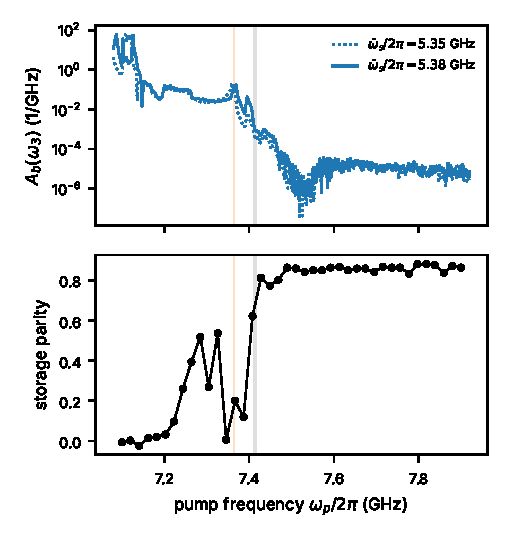
\includegraphics[width=\columnwidth]{fig_aws_cat.pdf}
\caption{\label{fig:cat}Filter-band heating channel in the cat qubit of Ref.~\cite{Putterman2025}. Top: filter weight
$A_b(\omega_3)$ at the leftover-photon frequency $\omega_3=2\omega_p-\bar\omega_s-2\bar\omega_b$, computed from the measured
filter transmission and the measured pumped buffer frequency, with no fitted parameter, for
$\bar\omega_s/2\pi=5.35$\,GHz (dotted) and $5.38$\,GHz (solid). The floor below $10^{-4}$ reflects the uncalibrated
out-of-band $S_{21}$. Bottom: measured storage parity averaged over $200$--$300\,\mu$s after the pump is switched on.
Grey band: $\omega_3$ leaves the filter's upper edge. Orange band: $\omega_3$ at the filter's upper-edge mode.}
\end{figure}

\end{document}
